\section{Uniform Convergence of a Sequence of Functions}

\begin{exercise}
  Let
  $$
  f_{n}(x)=\frac{n x}{1+n x^{2}} .
  $$
  \enum {
  \item Find the pointwise limit of $\left(f_{n}\right)$ for all $x \in(0, \infty)$.
  \item Is the convergence uniform on $(0, \infty)$?
  \item Is the convergence uniform on $(0,1)$?
  \item Is the convergence uniform on $(1, \infty)$?
  }
\end{exercise}
\begin{solution}
  \enum{
  \item $\lim f_n(x) = \lim \frac{nx}{1+nx^2} = \lim \frac{x}{1/n + x^2} = 1/x$
  \item Examine the difference $|f_n(x) - f(x)|$
    $$
    \left|\frac{nx}{1+nx^2} - \frac{1}{x}\right|
    = \left|\frac{nx^2 - (1+nx^2)}{x(1+nx^2)}\right|
    = \frac{1}{x(1+nx^2)}
    $$
    Consider $x_n = 1/n$, then
    $$
    \left|f_n(x_n) - f(x_n)\right| = \frac{1}{(1/n)(1+n(1/n^2)} = \frac{1}{n/2} = \frac{n}{2}
    $$
    Which shows that no matter how big $n$ is, we can find $x = 1/n$ such that $|f_n(x) - f(x)| \ge 1/2$ meaning $\epsilon$ cannot be made smaller then $1/2$. So $f$ isn't uniformly continuous.
  \item No, same logic as (b)
  \item Yes, because $x \ge 1$ implies
    $$
    |f_n(x) - f(x)| = \frac{1}{x(1 + nx^2)} \le \frac{1}{n}
    $$
    Meaning for all $\epsilon > 0$, setting $N > 1/\epsilon$ implies every $n \ge N$ has $|f_n(x) - f(x)| \le 1/N < \epsilon$ for every $x \in (1,\infty)$.
  }
\end{solution}
\begin{exercise}

  \enum {
  \item Define a sequence of functions on $\mathbf{R}$ by
    $$
    f_{n}(x)= \begin{cases}1 & \text { if } x=1, \frac{1}{2}, \frac{1}{3}, \ldots, \frac{1}{n} \\ 0 & \text { otherwise }\end{cases}
    $$
    and let $f$ be the pointwise limit of $f_{n}$.
    Is each $f_{n}$ continuous at zero? Does $f_{n} \rightarrow f$ uniformly on $\mathbf{R} ?$ Is $f$ continuous at zero?
  \item Repeat this exercise using the sequence of functions
    $$
    g_{n}(x)= \begin{cases}x & \text { if } x=1, \frac{1}{2}, \frac{1}{3}, \ldots, \frac{1}{n} \\ 0 & \text { otherwise. }\end{cases}
    $$
  \item Repeat the exercise once more with the sequence
    $$
    h_{n}(x)= \begin{cases}1 & \text { if } x=\frac{1}{n} \\ x & \text { if } x=1, \frac{1}{2}, \frac{1}{3}, \ldots, \frac{1}{n-1} \\ 0 & \text { otherwise. }\end{cases}
    $$
    In each case, explain how the results are consistent with the content of the Continuous Limit Theorem (Theorem 6.2.6).
  }
\end{exercise}
\begin{solution}
  \enum{
  \item Each $f_n$ is continuous at zero, but $f$ is not continuous at zero meaning (by Theorem 6.2.6) that $f_n$ does not converge to $f$ uniformly.
  \item Each $g_n$ is continuous at zero, and the pointwise limit $g$ is also continuous at zero. Since we aren't contradicting 6.2.6 the convergence may or may not be uniform.

    The definitions show $|g(x)-g_n(x)| < 1/n$ for all $x$ (max is at $x=1/(n+1)$).
    Setting $N > 1/\epsilon$ gives (for all $n \ge N$ and for all $x \in \mathbf{R}$)
    $$
    |g(x)-g_n(x)| < \epsilon
    $$
    As desired, thus $(g_n) \to g$ uniformly.
  \item Each $h_n$ is continuous at zero, and so is the pointwise limit $h$. 6.2.6 doesn't apply so we'll have to check if the convergence is uniform.
    Notice that if $x_n = 1/n$ then
    $$
    |h(x_n) - h_n(x_n)| = 1 - 1/n
    $$
    For all $n$, meaning no matter how big $n$ is, we can't make $|h-h_n|<1/2$ for all $x$ implying $h_n$ \emph{does not} converge to $h$ uniformly.
  }
\end{solution}
\begin{exercise}
  For each $n \in \mathbf{N}$ and $x \in[0, \infty)$, let
  $$
  g_{n}(x)=\frac{x}{1+x^{n}} \quad \text { and } \quad h_{n}(x)= \begin{cases}1 & \text { if } x \geq 1 / n \\ n x & \text { if } 0 \leq x<1 / n\end{cases}
  $$
  Answer the following questions for the sequences $\left(g_{n}\right)$ and $\left(h_{n}\right)$;
  \enum {
  \item Find the pointwise limit on $[0, \infty)$.
  \item Explain how we know that the convergence cannot be uniform on $[0, \infty)$.
  \item Choose a smaller set over which the convergence is uniform and supply an argument to show that this is indeed the case.
  }
\end{exercise}
\begin{solution}
  \enum{
  \item
    $$
    \lim g_n(x) = \begin{cases}
      x &\text{if } x \in [0, 1) \\
      \frac{1}{2} &\text{if } x = 1 \\
      0 &\text{if } x \in (1, \infty) \\
    \end{cases}
    \quad\text{and}\quad
    \lim h_n(x) = \begin{cases}
      1 &\text{if } x > 0 \\
      0 &\text{if } x = 0
    \end{cases}
    $$
  \item They can't converge uniformly since it would contradict Theorem 6.2.6 as both $g_n$ and $h_n$ are continuous but the limit functions are not.
  \item
    Over $[1,\infty)$ we have $h_n(x) = h(x) = 1$ for all $n$, thus $|h_n(x) - h(x)| = 0$ for all $x \in [1,\infty)$ so $h_n$ converges uniformly.

    Now for $g_n$. Let $t \in [0,1)$, I claim $g_n(x) \to x$ uniformly over $[0, t)$ since
    $$
    \left|\frac{x}{1 + x^n} - x\right|
    = \left|\frac{x - x(1+x^n)}{1 + x^n}\right|
    = \left|\frac{x^{n+1}}{1 + x^n}\right|
    < \left|t^{n+1}\right|
    < \epsilon \quad\forall x
    $$
    After setting $n > \log_t \epsilon$.
  }
\end{solution}

\begin{exercise}
  Review Exercise 5.2.8 which includes the definition for a uniformly differentiable function. Use the results discussed in Section 2 to show that if $f$ is uniformly differentiable, then $f^{\prime}$ is continuous.

\end{exercise}
\begin{solution}
  The definition of $f$ being uniformly differentiable tells us: for every $\epsilon > 0$ there exists a $\delta > 0$ such that
  $$
  \left|\frac{f(x)-f(y)}{x-y} - f'(y)\right| < \epsilon \quad \text{whenever $0<|x-y|<\delta$}
  $$
  We can use this to show continuity of $f'$ via a triangle inequality and exploiting the symmetry in $x,y$.
  $$
  |f'(x) - f'(y)|
  < \left|f'(x) - \frac{f(x)-f(y)}{x-y}\right|
  + \left|\frac{f(x)-f(y)}{x-y} - f'(y)\right|
  < \epsilon
  $$
  After picking $\delta$ so that every $|x-y|<\delta$ has
  $$
  \left|\frac{f(x)-f(y)}{x-y} - f'(y)\right| < \epsilon/2
  $$

  Alternative proof: Let \(y_n = x + 1/n\), and consider the sequence of functions
  \[f'_n(x) = \frac{f(x) - f(y_n)}{x - y_n}\]
  Each \(f'_n(x)\) is continuous, and uniform differentiability implies that \(f'_n\) uniformly converges to \(f'(x)\); hence \(f'(x)\) is continuous by Theorem 6.2.6.
\end{solution}
\begin{exercise}
  Using the Cauchy Criterion for convergent sequences of real numbers (Theorem 2.6.4), supply a proof for Theorem 6.2.5 (Cauchy Criterion for Uniform Convergence). (First, define a candidate for $f(x)$, and then argue that $f_{n} \rightarrow f$ uniformly.)

\end{exercise}
\begin{solution}
  In the forward direction, suppose $(f_n)$ converges uniformly to $f$ and set $N$ large enough that $n \ge N$ has $|f_n(x) - f(x)| < \epsilon/2$ for all $x$, then use the triangle inequality (where $m \ge N$ as well)
  $$
  |f_n(x) - f_m(x)| \le |f_n(x) - f(x)| + |f(x) - f_m(x)| < \epsilon/2 + \epsilon/2 = \epsilon.
  $$
  In the reverse direction, suppose we can find an $N$ so that every $n,m \ge N$ has $|f_n(x) - f_m(x)| < \epsilon /2$ for all $x$.
  Fix $x$ and apply Theorem 2.6.4 to conclude the sequence $(f_n(x))$ converges to some limit $L$, and define $f(x) = L$. Doing this for all $x$ gives us the pointwise limit $f$. Now we show $(f_n) \to f$ uniformly using the fact that $|f_n(x) - f_m(x)| < \epsilon / 2$ \emph{for all} $x$.
  Let $n \ge N$, notice that \emph{for all} $m$
  $$
  |f_n(x) - f(x)| \le |f_n(x) - f_m(x)| + |f_m(x) - f(x)|
  $$
  For all $m \ge N$ we have $|f_n(x) - f_m(x)| < \epsilon / 2$ and
  $$
  |f_n(x) - f(x)| < \epsilon/2 + |f_m(x) - f(x)|
  $$
  For any \(x\) we can choose \(m\) large enough to ensure $|f_m(x) - f(x)| < \epsilon / 2$ (pointwise convergence), and since the inequality is for all $m$ this implies $|f_n(x) - f(x)| \le \epsilon$ for all $x$ as desired.
\end{solution}
\begin{exercise}
  Assume $f_{n} \rightarrow f$ on a set $A$. Theorem 6.2.6 is an example of a typical type of question which asks whether a trait possessed by each $f_{n}$ is inherited by the limit function. Provide an example to show that all of the following propositions are false if the convergence is only assumed to be pointwise on $A$. Then go back and decide which are true under the stronger hypothesis of uniform convergence.
  \enum {
  \item If each $f_{n}$ is uniformly continuous, then $f$ is uniformly continuous.
  \item If each $f_{n}$ is bounded, then $f$ is bounded.
  \item If each $f_{n}$ has a finite number of discontinuities, then $f$ has a finite number of discontinuities.
  \item If each $f_{n}$ has fewer than $M$ discontinuities (where $M \in \mathbf{N}$ is fixed), then $f$ has fewer than $M$ discontinuities.
  \item If each $f_{n}$ has at most a countable number of discontinuities, then $f$ has at most a countable number of discontinuities.

  }
\end{exercise}
\begin{solution}
  \enum{
  \item False pointwise when
    $$
    f_n(x) = \frac{1}{1+nx^2} \quad\text{and}\quad f(x) = \begin{cases}
      1 &\text{if $x = 0$} \\
      0 &\text{otherwise}
    \end{cases}
    $$
    Now suppose $(f_n)$ converges to $f$ uniformly. We have
    \[|f(x) - f(y)| \leq |f(x) - f_n(x)| + |f_n(x) - f_n(y)| + |f_n(y) - f(y)| \]
    By uniform convergence to \(f\), we can fix \(n\) large enough so that the first and last terms are both less than \(\epsilon / 3\). Then since \(f_n\) is uniformly continuous, we can choose \(\delta\) so that \(|x - y| < \delta\) implies the middle term is less than \(\epsilon / 3\), and that \(|f(x) - f(y)| < \epsilon\), implying \(f\) is uniformly continuous.

  \item False pointwise when
    $$
    f_n(x)
    = \begin{cases}
      x &\text{if $x < n$} \\
      0 &\text{otherwise}
    \end{cases}
    \quad\text{and}\quad
    f(x) = x
    $$
    Now suppose $(f_n) \to f$ uniformly.
    We want to show $f$ is bounded.
    Let $M_n$ bound $f_n$, ie. $|f_n(x)|<M_n$ for all $x \in A$.

    Set $\epsilon=1$ and apply the Cauchy Criterion to get $N$ so $m \ge n > N$ implies
    $$
    |f_n(x) - f_m(x)| < 1
    $$
    Setting $n=N$ and rearranging gives
    $$
    |f_m(x)| < |f_N(x)| + \epsilon < M_N + \epsilon
    $$
    implying $f_m$ is bounded by $M_N$ when $m \ge N$.

    Now set $\tilde N > N$ large enough that $m \ge N$ implies $|f(x)-f_m(x)|<1$ which, after rearranging gives
    $$
    |f(x)| < 1 + |f_m(x)| < 1 + M_N
    $$
    Implying $f$ is bounded.
  \item False for pointwise and uniform convergence. Define
    $$
    f_n(x) = \begin{cases}
      1/m &\text{if $x = 1/m$ and $m\le n$, $m \in\mathbf{N}$} \\
      0 &\text{otherwise}
    \end{cases}
    $$
    and
    $$
    f(x) = \begin{cases}
      1/m &\text{if $x=1/m$, $m \in \mathbf{N}$} \\
      0 &\text{otherwise}
    \end{cases}
    $$
    The reason $(f_n) \to f$ uniformly is
    $$
    |f(x) - f_n(x)| = \left(
      \begin{cases}
        1/m &\text{if $x=1/m$ and $m > n$, $m \in \mathbf{N}$} \\
        0 &\text{otherwise}
      \end{cases}
    \right)
    < 1/{(n+1)}
    $$
    Each $f_n$ has exactly $n$ point discontinuities, but $f$ has countably many. Thus this is a counterexample.

    Intuitively $f_n$ adds on finer and finer details of $f$, which is why it converges uniformly. But discontinuities can be as small/detailed as we want without screwing up uniform convergence.
  \item False pointwise since we can have each $(f_n)$ continuous (zero discontinuities) but have $f$ not be continuous (see (a) for an example).

    Now suppose $(f_n) \to f$ uniformly. Let $x_0$ be a discontinuity of $f$, meaning there exists an $\epsilon_0$ such that $|f(x_0)-f(x)| > \epsilon_0$ no matter how small $|x-x_0|$ is.
    I'd like to show $x_0$ is a discontinuity of $f_n$ for some $n$, i.e.\ that there exists an $\epsilon_0'>0$ such that $|f_n(x_0)-f_n(x)|>\epsilon_0'$ no matter how small $|x-x_0|$ is.

    Pick $\epsilon<\epsilon_0/2$ and set $N$ large enough that $n \ge N$ implies $|f_n(x)-f(x)|<\epsilon$. Applying the three way triangle inequality gives
    $$
    \begin{aligned}
    \epsilon_0
    &< |f(x_0) - f(x)| \\
    &\le |f(x_0) - f_n(x_0)| + |f_n(x_0) - f_n(x)| + |f_n(x) - f(x)| \\
    &< 2\epsilon + |f_n(x_0) - f_n(x)|
    \end{aligned}
    $$
    Letting $\epsilon_0' = \epsilon_0-2\epsilon > 0$ we see $|f_n(x_0) - f_n(x)| > \epsilon_0'$ meaning $f_n$ is not continuous at $x_0$ for all $n \ge N$.

    Now given discontinuities of $f$, applying the above process multiple times shows that \emph{eventually} $f_n$ will have every discontinuity of $f$, but $f_n$ has at most $M$ discontinuities, implying $f$ has at most $M$ discontinuities.
  \item False pointwise when (using a modified version of Thomae's function for $f_n$)
    $$
    f_n(x) = \begin{cases}
      1 &\text{if $x = 0$} \\
      \frac{n}{n+q} &\text{if $x = p/q$ (in lowest terms)} \\
      0 &\text{otherwise}
    \end{cases}
    \quad\text{and}\quad
    f(x) = \begin{cases}
      1 &\text{if $x \in \mathbf{Q}$} \\
      0 &\text{if $x \notin \mathbf{Q}$} \\
    \end{cases}
    $$
    Now suppose $(f_n) \to f$ uniformly. In (d) we showed every discontinuity of $f$ is eventually a discontinuity of $f_n$; reworded this is saying (where $D_f$ is the set of discontinuities of $f$)
    $$
    D_f \subseteq \bigcup_{n=1}^\infty D_{f_{n}}
    $$
    Since each $D_{f_n}$ is countable, this implies $D_f$ is countable.
  }
\end{solution}
\begin{exercise}
  Let $f$ be uniformly continuous on all of $\mathbf{R}$, and define a sequence of functions by $f_{n}(x)=f\left(x+\frac{1}{n}\right)$. Show that $f_{n} \rightarrow f$ uniformly. Give an example to show that this proposition fails if $f$ is only assumed to be continuous and not uniformly continuous on $\mathbf{R}$.

\end{exercise}
\begin{solution}
  Given $\epsilon>0$ set $\delta>0$ such that $|x-y|<\delta$ implies $|f(x)-f(y)|<\epsilon$.
  Then set $N > 1/\delta$ so that $n \ge N$ implies (since $1/n<\delta$)
  $$
  |f(x) - f_n(x)| = |f(x) - f(x+1/n)| < \epsilon
  $$
  Which shows $(f_n) \to f$ uniformly.

  To see this doesn't work if $f$ is only continuous, consider $f(x) = x^2$.
  We have
\[
|f(x)-f_n(x)| = \abs{x^2 - \left(x + \frac{1}{n}\right)^2} = \abs{\frac{2x}{n} + \frac{1}{n^2}}
\]
  which given a fixed $n$, becomes arbitrarily big as $x$ goes to infinity. Hence $(f_n)$ does not converge uniformly.
\end{solution}
\begin{exercise}
  Let $\left(g_{n}\right)$ be a sequence of continuous functions that converges uniformly to $g$ on a compact set $K$. If $g(x) \neq 0$ on $K$, show $\left(1 / g_{n}\right)$ converges uniformly on $K$ to $1 / g$.

\end{exercise}
\begin{solution}
  Let's examine the difference
  $$
  |1/g(x) - 1/g_n(x)|
  = \left|\frac{g(x)-g_n(x)}{g(x)g_n(x)}\right|
  = \left|g(x)-g_n(x)\right|\left|\frac{1}{g(x)g_n(x)}\right|
  $$
  We'd like to bound the rightmost term.

  Theorem 6.2.6 implies $g$ is continuous, and Theorem 4.4.1 implies $g(K)$ is compact, hence $|g(K)|$ has a minimum, call it $m$. This allows us to bound $|1/g(x)| < 1/m$.

  To bound $1/g_n$ set $\epsilon$ small enough that $m-\epsilon>0$ then use uniform continuity to get $N$ such that $n \ge N$ has
  $$
  |g(x) - g_n(x)| < \epsilon
  $$
  Since $g_n(x) \in (g(x)-\epsilon, g(x)+\epsilon)$ we have $|g_n(x)| > |g(x)|-\epsilon$ and finally $|g(x)|>m$ implies $|g_n(x)|>m-\epsilon$ thus $|1/g_n(x)| < 1/(m-\epsilon)$ and so
  $$
  M = \frac{1}{m(m-\epsilon)} \implies |1/g(x) - 1/g_n(x)| < M|g(x)-g_n(x)|
  $$
  Given an $\epsilon$, setting $N$ big enough to make $|g(x)-g_n(x)| < M/\epsilon$ gives the desired result.
\end{solution}
\begin{exercise}
  Assume $\left(f_{n}\right)$ and $\left(g_{n}\right)$ are uniformly convergent sequences of functions.
  \enum {
  \item Show that $\left(f_{n}+g_{n}\right)$ is a uniformly convergent sequence of functions.
  \item Give an example to show that the product $\left(f_{n} g_{n}\right)$ may not converge uniformly.
  \item Prove that if there exists an $M>0$ such that $\left|f_{n}\right| \leq M$ and $\left|g_{n}\right| \leq M$ for all $n \in \mathbf{N}$, then $\left(f_{n} g_{n}\right)$ does converge uniformly.

  }
\end{exercise}
\begin{solution}
  \enum{
  \item Obvious by the triangle inequality and Cauchy Criterion
  \item Let $f_n(x) = x = f(x)$ and $g_n(x) = x+1/n$. Suppose $n,m \ge N$ for some $N$, Cauchy gives us
    $$
    |f_ng_n - f_mg_m| = |x(1/n - 1/m)|
    $$
    Making $x$ large makes the error blow up regardless of how big $N$ is, thus $f_ng_n$ does not converge uniformly.
  \item By the triangle inequality (same trick as for the product rule)
    $$
    \begin{aligned}
      |f_ng_n - f_mg_m|
      &\le |f_ng_n - f_ng_m| + |f_ng_m - f_mg_m| \\
      &= |f_n|\cdot|g_n - g_m| + |g_m|\cdot |f_n-f_m| \\
      &< M|g_n - g_m| + M|f_n-f_m| \\
      &< \epsilon/2 + \epsilon/2 = \epsilon
    \end{aligned}
    $$
    After setting $N$ big enough that $n,m \ge N$ implies $|f_n-f_m|<M/2\epsilon$ and $|g_n-g_m|<M/2\epsilon$.
  }
\end{solution}
\begin{exercise}
  This exercise and the next explore partial converses of the Continuous Limit Theorem (Theorem 6.2.6). Assume $f_{n} \rightarrow f$ pointwise on $[a, b]$ and the limit function $f$ is continuous on $[a, b]$. If each $f_{n}$ is increasing (but not necessarily continuous), show $f_{n} \rightarrow f$ uniformly.


\end{exercise}
\begin{solution}
\(f\) is continuous and therefore will map \([a, b]\) to a closed interval \([c, d]\). By the Order Limit Theorem, we also know that \(f\) must be increasing - just compare the sequence \(\lim_{n \to \infty} f_n(x_1)\) to \(\lim_{n \to \infty} f_n(x_2)\) when \(x_2 > x_1\).

The key implication of \(f_n\) and \(f\) being increasing is that there is a bound to how fast the error \(\abs{f - f_n}\) can grow with respect to \(x\), which is proportional to how fast \(f\) grows. Intuitively, if we have \(f > f_n\) and want the error to grow as fast as possible with respect to \(x\), all we can do is hold \(f_n\) constant. Alternatively, if we have \(f < f_n\), \(f_n\) can't go too far above \(f\) since \(f\) needs to catch up eventually.

More formally, for \(\epsilon > 0\), define \(y_1, y_2, y_3, \dots, y_n\) to evenly split up \([c, d]\) into intervals of size at most \(\epsilon_1 = \epsilon / 5\). (In other words, \(y_1 = c\), \(y_n=d\), \(y_{k+2} - y_{k+1} = y_{k+1} - y_k < \epsilon_1\).) Since \(f\) is increasing, we can define \(x_1, \dots, x_n\) so that \(f(x_k) = y_k\).

Since \(f_n \to f\), we can find \(M_k\) so that \(m_k > M_k\) implies \(\abs{y_k - f_{m_k}(x_k)} < \epsilon_1\). Let \(M = \max\{M_1, M_2, \dots, M_n\}\). Now, let \(m > M\) be arbitrary.
 Keeping in mind that \(f_m\) is increasing, we can bound \(f_m(x_{i+1}) - f_m(x_i)\) by
\[ \begin{aligned}
f_m(x_{i+1}) - f_m(x_i) &= |f_m(x_{i+1}) - f_m(x_i)| \\
    &\leq |f_m(x_{i+1}) - y_{i+1}| + |y_{i+1} - y_i| + |y_i - f_m(x_i)| \\
    &< \epsilon_1 + \epsilon_1 + \epsilon_1 = 3 \epsilon_1
\end{aligned} \]

Now consider \(\abs{f(x) - f_m(x)} \quad x \in [x_i, x_{i+1}]\) with \(i\) arbitrary.
 Since \(f\) is increasing, \(y_i \leq f(x) \leq y_{i+1}\), so \(f(x) - y_i < \epsilon_1\). Similarly \(f_m(x) - f_m(x_i) \leq f_m(x_{i+1}) - f_m(x_i) < 3\epsilon_1\). Finally, we have
 \[\begin{aligned}
 \abs{f(x) - f_m(x)} &= \abs{f(x) - y_i} + \abs{y_i - f_m(x_i)} + \abs{f_m(x) - f_m(x_i)} \\
 &< \epsilon_1 + \epsilon_1 + 3\epsilon_1 = \epsilon
 \end{aligned} \]
 Since \(m\) and \(i\) were arbitrary, this completes the proof.
\end{solution}

\begin{exercise}[Dini's Theorem]
  Assume $f_{n} \rightarrow f$ pointwise on a compact set $K$ and assume that for each $x \in K$ the sequence $f_{n}(x)$ is increasing. Follow these steps to show that if $f_{n}$ and $f$ are continuous on $K$, then the convergence is uniform.
  \enum {
  \item Set $g_{n}=f-f_{n}$ and translate the preceding hypothesis into statements about the sequence $\left(g_{n}\right)$.
  \item Let $\epsilon>0$ be arbitrary, and define $K_{n}=\left\{x \in K: g_{n}(x) \geq \epsilon\right\} .$ Argue that $K_{1} \supseteq K_{2} \supseteq K_{3} \supseteq \cdots$, and use this observation to finish the argument.
  }
\end{exercise}
\begin{solution}
  \enum{
  \item We want $(g_n) \to 0$ uniformly, where $g_n$ is continuous, $g_n(x)$ is decreasing and $g_n(x) \to 0$.
  \item $x \in K_{n+1}$ by definition has $g_{n+1}(x) \ge \epsilon$, since $(g_n(x))$ is decreasing we must also have $g_{n}(x) \ge \epsilon$. Thus $K_{n+1} \subseteq K_n$. Now, if each $K_n \ne \emptyset$ the nested compact set property (Theorem 3.3.5) would imply there exists an $x_0 \in \bigcap_{n=1}^\infty K_n$. But this is impossible because $g_n(x_0) \to 0$ implies eventually $g_n(x_0)<\epsilon$.
    Therefore since the compact set property doesn't apply, there must exist an $N$ with $K_N = \emptyset$, implying every $n \ge N$ has (by subsets) $K_n = \emptyset$ and thus $|g_n| < \epsilon$.
  }
  % TODO: Understand intuitively, I proved it but I have no idea why it's true
\end{solution}
\begin{exercise}[Cantor Function]
  Review the construction of the Cantor set $C \subseteq[0,1]$ from Section 3.1. This exercise makes use of results and notation from this discussion.
  \enum {
  \item Define $f_{0}(x)=x$ for all $x \in[0,1]$. Now, let
    $$
    f_{1}(x)= \begin{cases}(3 / 2) x & \text { for } 0 \leq x \leq 1 / 3 \\ 1 / 2 & \text { for } 1 / 3<x<2 / 3 \\ (3 / 2) x-1 / 2 & \text { for } 2 / 3 \leq x \leq 1\end{cases}
    $$
    Sketch $f_{0}$ and $f_{1}$ over $[0,1]$ and observe that $f_{1}$ is continuous, increasing, and constant on the middle third $(1 / 3,2 / 3)=[0,1] \backslash C_{1}$.
  \item Construct $f_{2}$ by imitating this process of flattening out the middle third of each nonconstant segment of $f_{1}$. Specifically, let
    $$
    f_{2}(x)= \begin{cases}(1 / 2) f_{1}(3 x) & \text { for } 0 \leq x \leq 1 / 3 \\ f_{1}(x) & \text { for } 1 / 3<x<2 / 3 \\ (1 / 2) f_{1}(3 x-2)+1 / 2 & \text { for } 2 / 3 \leq x \leq 1\end{cases}
    $$
    If we continue this process, show that the resulting sequence $\left(f_{n}\right)$ converges uniformly on $[0,1]$.
  \item Let $f=\lim f_{n}$. Prove that $f$ is a continuous, increasing function on $[0,1]$ with $f(0)=0$ and $f(1)=1$ that satisfies $f^{\prime}(x)=0$ for all $x$ in the open set $[0,1] \backslash C$. Recall that the ``length'' of the Cantor set $C$ is 0 . Somehow, $f$ manages to increase from 0 to 1 while remaining constant on a set of ``length 1.''

  }
\end{exercise}
\begin{solution}
  \enum{
  \item \(f_0\) in red, \(f_1\) in blue:

  \begin{figure}[h]
    \centering
    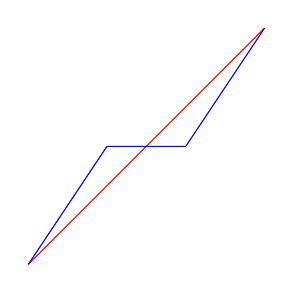
\begin{tikzpicture}[scale=3]
      \draw[red](0,0) -- (1, 1);
      \draw[blue] (0, 0)   -- (1/3, 1/2) -- (2/3, 1/2) -- (1, 1);
    \end{tikzpicture}
  \end{figure}
  \item \TODO I think we want to somehow apply the previous exercise, but I don't see how we can show $f$ is continuous... Maybe Cauchy is the way to go?
  \item \TODO
  }
\end{solution}
\begin{exercise}
  Recall that the Bolzano-Weierstrass Theorem (Theorem 2.5.5) states that every bounded sequence of real numbers has a convergent subsequence. An analogous statement for bounded sequences of functions is not true in general, but under stronger hypotheses several different conclusions are possible. One avenue is to assume the common domain for all of the functions in the sequence is countable. (Another is explored in the next two exercises.)
  Let $A=\left\{x_{1}, x_{2}, x_{3}, \ldots\right\}$ be a countable set. For each $n \in \mathbf{N}$, let $f_{n}$ be defined on $A$ and assume there exists an $M>0$ such that $\left|f_{n}(x)\right| \leq M$ for all $n \in \mathbf{N}$ and $x \in A$. Follow these steps to show that there exists a subsequence of $\left(f_{n}\right)$ that converges pointwise on $A$.

  \enum {
  \item Why does the sequence of real numbers $f_{n}\left(x_{1}\right)$ necessarily contain a convergent subsequence $\left(f_{n_{k}}\right)$ ? To indicate that the subsequence of functions $\left(f_{n_{k}}\right)$ is generated by considering the values of the functions at $x_{1}$, we will use the notation $f_{n_{N}}=f_{1, k}$.
  \item Now, explain why the sequence $f_{1, k}\left(x_{2}\right)$ contains a convergent subsequence.
  \item Carefully construct a nested family of subsequences $\left(f_{m, k}\right)$, and show how this can be used to produce a single subsequence of $\left(f_{n}\right)$ that converges at every point of $A$.

  }
\end{exercise}
\begin{solution}
  \TODO
\end{solution}
\begin{exercise}
  A sequence of functions $\left(f_{n}\right)$ defined on a set $E \subseteq \mathbf{R}$ is called equicontinuous if for every $\epsilon>0$ there exists a $\delta>0$ such that $\left|f_{n}(x)-f_{n}(y)\right|<\epsilon$ for all $n \in \mathbf{N}$ and $|x-y|<\delta$ in $E$.
  \enum {
  \item What is the difference between saying that a sequence of functions $\left(f_{n}\right)$ is equicontinuous and just asserting that each $f_{n}$ in the sequence is individually uniformly continuous?
  \item Give a qualitative explanation for why the sequence $g_{n}(x)=x^{n}$ is not equicontinuous on $[0,1]$. Is each $g_{n}$ uniformly continuous on $[0,1]$ ?

  }
\end{exercise}
\begin{solution}
  \enum{
  \item For equicontinuous functions the same $\delta$ works for every function in the sequence, as opposed to individually being uniformly continuous where $\delta$ depends on $n$.
  \item Not equicontinuous since as $n$ increases we need $\delta$ to be smaller, hence $\delta$ cannot be written independent of $n$. Each $g_n$ is uniformly continuous however (since $g_n$ is continuous on the compact set $[0,1]$).
  }
\end{solution}
\begin{exercise}[Arzela-Ascoli Theorem]
  For each $n \in \mathbf{N}$, let $f_{n}$ be a function defined on $[0,1]$. If $\left(f_{n}\right)$ is bounded on $[0,1]$-that is, there exists an $M>0$ such that $\left|f_{n}(x)\right| \leq M$ for all $n \in \mathbf{N}$ and $x \in[0,1]$-and if the collection of functions $\left(f_{n}\right)$ is equicontinuous (Exercise 6.2.14), follow these steps to show that $\left(f_{n}\right)$ contains a uniformly convergent subsequence.
  \enum {
  \item Use Exercise 6.2.13 to produce a subsequence $\left(f_{n_{k}}\right)$ that converges at every rational point in $[0,1]$. To simplify the notation, set $g_{k}=f_{n_{k}}$. It remains to show that $\left(g_{k}\right)$ converges uniformly on all of $[0,1]$.
  \item Let $\epsilon>0$. By equicontinuity, there exists a $\delta>0$ such that
    $$
    \left|g_{k}(x)-g_{k}(y)\right|<\frac{\epsilon}{3}
    $$
    for all $|x-y|<\delta$ and $k \in \mathbf{N}$. Using this $\delta$, let $r_{1}, r_{2}, \ldots, r_{m}$ be a finite collection of rational points with the property that the union of the neighborhoods $V_{\delta}\left(r_{i}\right)$ contains $[0,1]$.
    Explain why there must exist an $N \in \mathbf{N}$ such that
    $$
    \left|g_{s}\left(r_{i}\right)-g_{t}\left(r_{i}\right)\right|<\frac{\epsilon}{3}
    $$
    for all $s, t \geq N$ and $r_{i}$ in the finite subset of $[0,1]$ just described. Why does having the set $\left\{r_{1}, r_{2}, \ldots, r_{m}\right\}$ be finite matter?
  \item Finish the argument by showing that, for an arbitrary $x \in[0,1]$,
    $$
    \left|g_{s}(x)-g_{t}(x)\right|<\epsilon
    $$
    for all $s, t \geq N$.
  }
\end{exercise}
\begin{solution}
  \TODO
\end{solution}
